\chapter{Introducci\'on}

Actualmente, los dispositivos de video capturan una gran cantidad de informaci\'on de escenas del mundo real para que sean procesadas en sistemas de c\'omputo. Esto ha motivado un incremento en los servicios de video tales como aplicaciones de \textit{broadcasting}, \textit{streaming} en vivo, video-chat, videoconferencia, video en redes m\'oviles entre otros. La evoluci\'on de estos servicios crean fuertes necesidades en t\'erminos de ancho de banda y procesamiento, especialmente para contenido en alta definici\'on, como 1080p, y contenido de ultra alta definici\'on, como 4k y 8k. Con estos nuevos avances se incrementa dr\'asticamente la informaci\'on necesaria para representar un video, especialmente para la transmisi\'on como se puede observar en la Fig. \ref{fig:vni}.

\begin{figure}[!h]
\centering
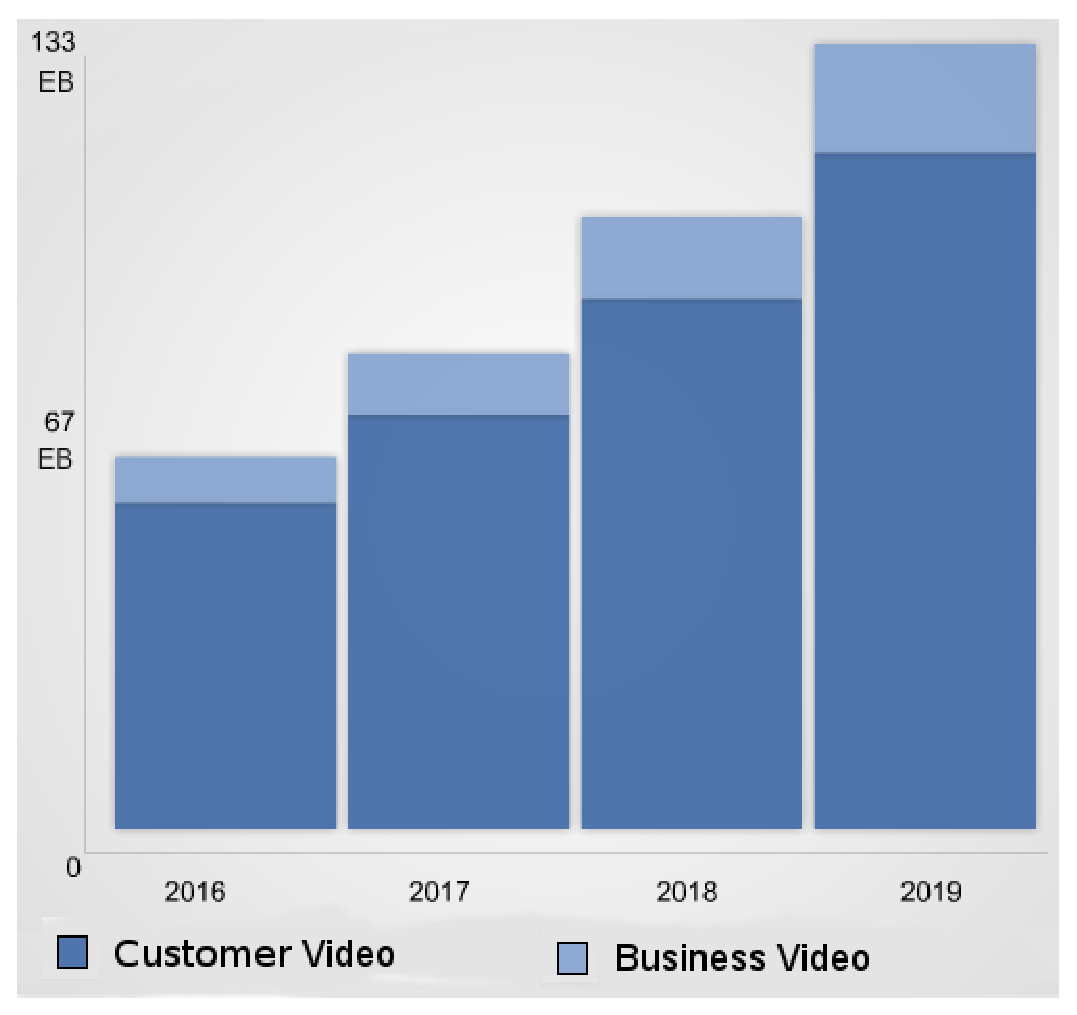
\includegraphics[width=0.4\textwidth]{images/vni.eps}
\caption[Crecimiento estimado de tr\'afico de video por Internet IP]{Crecimiento estimado de tr\'afico de video por Internet IP \cite{cisco_vni}} 
\label{fig:vni}
\end{figure}

Para atender estos requerimientos, se han incrementado los esfuerzos en la creaci\'on de propuestas de codificaci\'on de video para mejorar la eficicencia de codificaci\'on, es decir, que con la menor cantidad de bits se pueda representar un video con cierta calidad, teniendo en cuenta la complejidad computacional y un retraso entre el proceso de codificaci\'on y decodificaci\'on. Actualmente uno de los avances m\'as importantes en codificac\'on de video es el estandar de codificaci\'on de video de alta eficiencia (HEVC) \cite{hevc}, desarrollado conjuntamente por los grupos ITU-T VCEG\footnote{Grupo de Expertos en Codificaci\'on de Video de la Union Internacional de Telecomunicaciones - Sector de Estandarizaci\'on de Telecomunicaciones Internacional} y ISO/IEC MPEG\footnote{Grupo de Expertos de Im\'agenes en Movimiento de Organizaci\'on Internacional
de Normalizaci\'on y la Comisi\'on Electrot\'ecnica Internacional}. Con el HEVC se logr\'o mejorar la eficiencia de codificaci\'on, reduciendo la tasa de bits aproximadamente un 50\% en comparaci\'on con su antecesor, el est\'andar de codificaci\'on H.264 \cite{wiegand_overview_2003}, aunque en t\'erminos de complejidad computacional hay un incremento significativo \cite{6317156}. Otra apuesta importante de codificaci\'on de video es el est\'andar de codificaci\'on de c\'odigo libre desarrollado por Google denominado VP9, el cual se centra en la compresi\'on de contenido de alta definici\'on \cite{6737765}.

Los est\'andares de codificaci\'on explotan la correlaci\'on espacial y temporal entre frames de un video, y en los \'ultimos a\~nos, las t\'ecnicas de \textit{Compressed Sensing} (CS) han emergido como un enfoque para simplificar la representaci\'on de la se\~nal, aprovechando la propiedad de dispersi\'on (\textit{sparsity}), la cual indica que la mayoria de coeficientes de un vector son cero. Las t\'ecnicas de CS usan un peque\~no numero de muestras para reconstruir una se\~nal resolviendo un problema de minimizaci\'on de la norma $\ell_p$ mediante un diccionario de muestras \cite{compressive}. Uno de los elementos fundamentales para el CS es la selecci\'on del diccionario, ya que con un buen diccionario se pueden garantizar una mejor reconstrucci\'on de una se\~nal. Para la selecci\'on del diccionario se pueden usar muestras extra\'idas directamente de la se\~nal  o se puede realizar un entrenamiento para que se adapte a las condiciones de la se\~nal. Otra propuesta que ha tomado fuerza en los \'ultimos a\~nos es la codificaci\'on de video perceptual, donde se tienen en cuenta caracter\'isticas perceptuales del Sistema Visual Humano (HVS), que pueden ser modeladas computacionalmente y de esta forma mejorar la eficiencia de codificaci\'on en t\'erminos de la degradaci\'on de la calidad a un nivel que apenas pueda ser percibido por el ojo humano \cite{yu-bei_lin_recent_2013}.

Este documento presenta una propuesta para seleccionar el diccionario de un modelo para CS usando m\'etodos de codificaci\'on perceptual. El documento esta organizado de la siguiente manera, en el cap\'itulo \ref{chap:problem} se presenta la descripci\'on del problema, los objetivos del proyecto y la justificaci\'on de la propuesta. En el cap\'itulo \ref{chap:background} se presenta el marco conceptual sobre  codificaci\'on de video y \textit{compressed sensing}.  En el cap\'itulo \ref{chap:related} se presenta un estado del arte que incluye los algoritmos de entrenamiento de diccionarios, propuestas de codificaci\'on de video con t\'ecnicas de CS, m\'etodos de codificaci\'on perceptual y propuestas de codificaci\'on de video con CS y codificaci\'on perceptual. En el cap\'itulo \ref{chap:proposed} se describe el enfoque que se desea proponer en el proyecto. Finalmente, en el cap\'itulo \ref{chap:methodology} se presenta la metodolog\'ia que se va a usar en el proyecto, las actividades a desarrollar y el cronograma. 
